\section{Requisitos}
Como la metodología de desarrollo ha sido iterativa, algunos de los requisitos han ido surgiendo durante el desarrollo de la aplicación, e inclusos algunos requisitos han cambiado según se han ido encontrando o destruyendo barreras. Los requisitos iniciales, que se plantearon en la primera reunión eran:

Desarrollar una aplicación para cuatro jugadores en las que compiten para encontrar la palabra. En este momento ya se ha definido que es un juego variante del Wordle, además, por simplificar el desarrollo en estos momentos iniciales, se ha decidido guardar la información sobre los jugadores en memoría, sin utilizar ninguna base de datos.

\subsection{Fases}
En cada fase de desarrollo quedan agrupadas una serie de nuevos requisitos y mejoras sobre los requisitos que ya se habían completado.

\subsubsection{Fase 0}
En la fase 0, se propone la idea de la aplicación y se comienzan a crear requisitos, primero se define las ideas y los requerimientos, como la necesidad de crear un sistema de tiempo real, además, se especifican las tecnologías, y se define como debería de avanzar el proyecto a lo largo del tiempo.

\subsubsection{Fase 1}
En la fase 1, se presentó una primera versión de la aplicación, en ella un número no controlado de jugadores podían jugar en una misma sala, existía un lobby donde los jugadores podían cambiar su nombre y podían jugar hasta que uno ganase. Todavía no se llegaba a controlar el que los jugadores hubieran perdido, así que era posible quedarse bloqueado con todos los jugadores sin posibilidad de probar nuevas palabras.
La palabra objetivo en esta fase no era generada aleatoriamente, en su lugar, era siempre la misma palabra. Esto facilitaba mucho las pruebas iniciales de flujo de la aplicación.

\subsubsection{Fase 2}
En la fase 2, el servidor ya era capaz de generar una palabra aleatoria entre una lista de posibles palabras. Todos los jugadores reciben la palabra objetivo aleatoria al comenzar la partida, en el momento en el que uno de ellos ganaba, se mostraba su nombre y la palabra objetivo en una nueva página.
	      	      	      	      	      	      	      	      
La página que muestra al jugador ganador, como el resto de páginas, fue cambiando a lo largo del tiempo, sobre ella se hicieron muchas iteraciones que permitieron llegar al diseño final.

\subsubsection{Fase 3}
En la fase 3, se introdujo la opción de unir a traves del boton de Join del menú principal, además, se introdujo la posibilidad de ver en tiempo real el conocimiento adquirido de cada jugador sobre la palabra objetivo y se amplió la lista de palabras para que soportara diferentes idiomas, en concreto se introdujo el idioma español, pero el sistema es capaz de introducir nuevas listas de palabras de manera sencilla.
	      	      	      	      
Además, se prestó especial atención a casos donde hay un único jugador en la partida, por ejemplo, para estos casos se eliminó la cuenta atrás del principio de la partida.
	      	      	      	      	
Para poder probar con amigos y compañeros de trabajo, se desplegó la aplicación moviendo las aplicaciones a un servidor de DigitalOcean, levantando ambas aplicaciones utilizando los comandos que proveen tanto SvelteKit como Deno. Esta forma de levantar las aplicaciones se demostró muy lenta, ya que requería actualizar los repositorios del servidor usando Git, para después compilar y ejecutar las aplicaciones.

\subsubsection{Fase 4} Para la fase 4, se arreglaron bugs presentes, además se desarrolló la posibilidad de levantar la aplicación utilizando Docker y Docker Compose.

En este momento la aplicación ya se encontraba con madurez suficiente para que los cambios necesarios fueran aplicados sin necesidad de hacer refactorizaciones ni grandes cambios en los sistemas de la aplicación.    	      	      	      	      	


\section{Arquitectura general}
El proyecto está dividido en dos repositorios, por un lado está la aplicación web (webapp), que se encarga de realizar la lógica de presentación, así como el game loop, y por otro lado tenemos el servidor de backend, donde va toda la lógica de websockets en la parte de servidor.

La comunicación entre aplicaciones se realiza mediante peticiones HTTP y websockets, para ello se utiliza la librería estándar de Javascript proporcionada por el navegador, la librería estándar de Node.js, la librería estándar de Deno y la librería Socket.io.


\begin{center}
	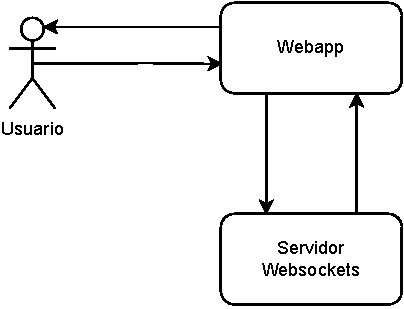
\includegraphics[clip=true,width=0.5\textwidth]{./diagrams/general_arch.pdf}
\end{center}

\subsection{Aplicación web}
La aplicación web es la herramienta con la cual el usuario interactúa, permite a este realizar todas las acciones necesarias utilizando un navegador web.

Está desarrollada utilizando SvelteKit para la realización de la lógica, y Tailwind para dar color y estilo.

El flujo principal que sigue el usuario para poder jugar una partida comienza abriendo la página web de la aplicación web, después, creará o se unirá a una partida ya creada, cuando todos los jugadores estén listos, el creador de la partida le dará al botón de comenzar, y después de una cuenta atrás, a todos los jugadores se les presentará un tablero de Wordle donde pondrán ir escribiendo sus intentos. Si alguno de los jugadores descubre la palabra, todos los jugadores verán una nueva pantalla con el nombre de la persona ganadora, en esta nueva pantalla, los jugadores pueden elegir entre salir de la partida o volver a jugar. En caso de que ningún jugador consiga ganar, se les presentará a todos una pantalla en el que se mostrará la palabra objetivo, y las mismas opciones que en el caso de haber habido un ganador.


\begin{center}
	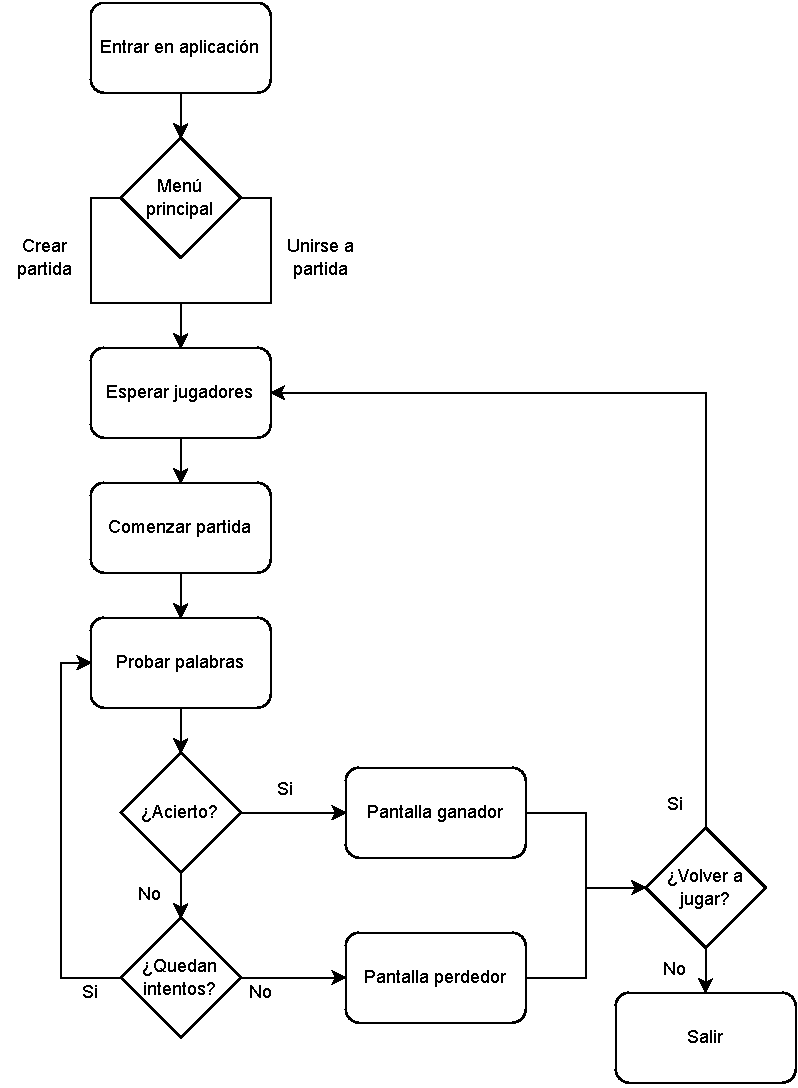
\includegraphics[clip=true,width=\textwidth]{./diagrams/webapp_flow.pdf}
\end{center}


\subsection{Servidor Websockets}

El servidor de websockets está implementado utilizando Deno y una librería que ayuda al manejo de eventos para los websockets llamada Socket.io. Deno se utiliza para levantar el servidor y para recibir peticiones HTTP, aunque existen pocos endpoints para la comunicación HTTP, existe un endpoint necesario para que Socket.io cree la conexión de Websockets, y uno más para la creación de la partida.

\subsubsection{Endpoints disponibles}

El servidor permite la comunicación utilizando las siguientes rutas HTTP:Soso

\begin{itemize}
	\item \textit{/create-route}, genera un nuevo identificador de partida. Este identificador es fundamental para la comunicación entre el cliente y el servidor ya que permite la identificación de la partida para realizar las operaciones necesarias.
	\item \textit{/testing/solution}, este endpoint está disponible para poder realizar un tests de integración de flujo completo.correcta.
\end{itemize}

A parte de las rutas HTTP, el servidor permite la comunicación Websocket utilizando los siguientes eventos:

\begin{itemize}
	\item \textit{setup} es un evento de tipo diálogo que une a un jugador a la partida, es necesario enviar como parámetros el código de la sala generado por /create-room y el nombre del usuario que se va a unir a la partida, este evento avisa a todos los demás jugadores de la sala que se ha unido el jugador emitiendo el evento \textit{player\_connection}.
	\item \textit{update\_player\_name} es un evento de tipo diálogo que permite a los jugadores actualizar su nombre, especialmente útil porque el primer nombre que recibe cada jugador al conectarse a la partida es aleatorio entre una combinación de posibilidades.
	\item \textit{remove\_player} es un evento de tipo out que solo pueden utilizar el creador de la partida, y permite expulsar a jugadores de la partida. Cuando ha expulsado a un jugador emite un evento \textit{player\_disconnected} que notifica al resto de usuarios de la desconexión.
	\item \textit{validate\_word} es un evento de tipo diálogo que comprueba un intento de un jugador con la palabra objetivo. El resultado de la operación de comprobación es un array de una enumeración (\textit{WordlePoints}) que indican el resultado de cada letra en la palabra (si no se encuentra en la palabra, si se encuentra en la palabra, si está en la posición correcta). Este resultado se envía directamente al jugador que ha ejecutado el evento, pero también se envía a los demás jugadores para indicar en el scoreboard el conocimiento de cada jugador. Además, se comprueba si la partida ha terminado por que el intento coincide con la palabra objetivo, y si todos los jugadores han perdido porque se han quedado sin intentos.
	\item \textit{start\_game} es un evento de tipo out que permite al host de la partida empezar. En el momento que se lanza este evento todos los jugadores reciben el evento \textit{start\_prematch} que les indica cuándo comenzará la partida.
	\item \textit{disconnect} es un evento nativo de Socket.io, que permite al servidor conocer cuando un jugador se ha desconectado de la partida, existen varias razones para que se ejecute este evento, por ejemplo, que el jugador haya perdido la conexión con internet, o que el jugador haya decidido abandonar la partida cerrando el navegador. En este evento se comunica al resto de jugadores que este ha abandonado la partida, en caso de ser el jugador que ha creado la partida el que la abandona, se cierra también para el resto de jugadores.
\end{itemize}
